%-----------------------------------------------------------------------------%
\chapter{\babEmpat}
%-----------------------------------------------------------------------------%

Bab ini membahas hasil simulasi dan analisis kinerja model \textit{Joint
Sentiment-Topic} berbasis \textit{multitask learning} yang diusulkan.
Data yang digunakan berasal dari dataset IMDB dan Yelp yang telah melalui
tahap prapengolahan dan pembagian data. Kinerja model dievaluasi dari dua
aspek, yaitu analisis sentimen dan pendeteksian topik. Pada analisis
sentimen, performa diukur menggunakan metrik \textit{accuracy},
\textit{precision}, \textit{recall}, dan \textit{F1-score}. Pada
pendeteksian topik, kualitas topik dinilai menggunakan metrik
\textit{Topic Coherence} berbasis NPMI dan \textit{Topic Diversity}.
Hasil interpretasi model melalui analisis atribusi token juga dipaparkan
untuk menggambarkan karakteristik linguistik tiap klaster topik.

%-----------------------------------------------------------------------------%
\section{Spesifikasi Mesin dan Perangkat Lunak}
%-----------------------------------------------------------------------------%

Spesifikasi mesin dan perangkat lunak yang digunakan dalam proses simulasi
pada penelitian ini dapat dilihat pada Tabel~\ref{tab:spesifikasi}.

\begin{table}[H]
    \centering
    \caption{Spesifikasi mesin dan perangkat lunak}
    \label{tab:spesifikasi}
    \begin{tabular}{|l|l|}
        \hline
        \multicolumn{2}{|c|}{\textbf{Mesin}} \\
        \hline
        \textit{Central Processing Unit} (CPU) & Apple M1 \\
        \hline
        \textbf{Memory}                        & 8 GB \\
        \hline
        \textit{Graphic Processing Unit} (GPU) & Apple M1 GPU (8-core) \\
        \hline
        \multicolumn{2}{|c|}{\textbf{Perangkat Lunak}} \\
        \hline
        Perangkat Lunak Pemrograman &
            Google Colaboratory \\
                                    &
            Kaggle Notebooks \\
                                    &
            Visual Studio Code \\
        \hline
        Bahasa Pemrograman          & Python 3.13.3 \\
        \hline
        Pustaka yang Digunakan      &
            \begin{tabular}[t]{@{}ll@{}}
                - os, re, csv, json, glob & - transformers \\
                - numpy, pandas           & - datasets \\
                - PyTorch (torch)         & - tqdm \\
                - scikit-learn, scipy     & - seaborn \\
            \end{tabular} \\
        \hline
    \end{tabular}
\end{table}

%-----------------------------------------------------------------------------%
\section{Tahapan Umum Simulasi}
%-----------------------------------------------------------------------------%

Tahapan umum simulasi pada penelitian ini digambarkan dalam diagram alur
pada Gambar~\ref{fig:alur_simulasi}.

\begin{figure}[H]
    \centering
    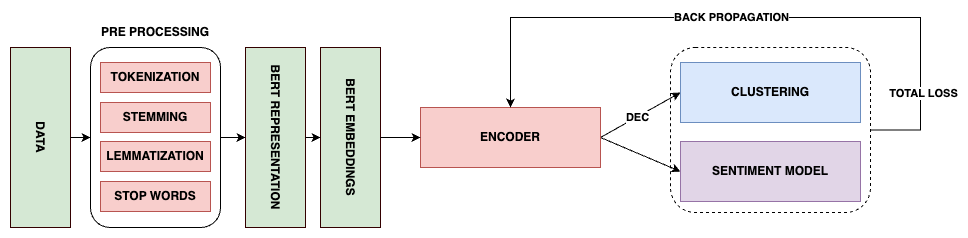
\includegraphics[width=0.85\textwidth]{assets/pics/MTL/FNN1.png}
    \caption{Diagram alur simulasi penelitian.}
    \label{fig:alur_simulasi}
\end{figure}

Proses dimulai dengan pengumpulan data ulasan yang kemudian melewati tahap
prapengolahan untuk menghasilkan data yang bersih. Data tersebut selanjutnya
diproses oleh BERT yang digunakan secara \textit{feature-based} dengan bobot
yang dibekukan, menghasilkan representasi vektor \texttt{[CLS]} berdimensi
768 untuk setiap dokumen. Representasi ini kemudian menjadi masukan bagi
\textit{autoencoder} untuk menghasilkan representasi laten berdimensi lebih
rendah.

Representasi laten yang dihasilkan digunakan secara bersamaan oleh dua jalur
tugas, yaitu analisis sentimen melalui \textit{sentiment head} dan
pendeteksian topik melalui \textit{Deep Embedded Clustering} (DEC). Setelah
pelatihan \textit{joint} selesai, kinerja dari kedua tugas dievaluasi dengan
metrik yang sesuai.

%-----------------------------------------------------------------------------%
\section{Data}
%-----------------------------------------------------------------------------%

Subbab ini menjelaskan data yang digunakan dalam penelitian, meliputi sumber
data, karakteristik dataset, serta tahapan persiapan data sebelum digunakan
dalam pelatihan model. Secara umum, proses pengolahan data dimulai dari
pengumpulan dataset ulasan, lalu dilanjutkan dengan prapengolahan teks,
pembentukan representasi menggunakan BERT, dan pembagian data.

%-----------------------------------------------------------------------------%
\subsection{Pengumpulan Data}
%-----------------------------------------------------------------------------%

Penelitian ini menggunakan dua dataset ulasan berbahasa Inggris, yaitu IMDB
Movie Reviews dan Yelp Review Dataset. Kedua dataset dipilih karena umum
digunakan sebagai \textit{benchmark} pada penelitian analisis sentimen dan
pendeteksian topik, serta keduanya memiliki label sentimen biner.

Dataset IMDB Movie Reviews terdiri dari 30.000 ulasan film yang diunggah oleh
\parencite{maas2011} dan tersedia secara publik melalui platform Hugging Face
dalam format Apache Arrow. Distribusi label sentimen pada dataset ini relatif
seimbang antara kelas positif dan negatif, sehingga cocok untuk tugas
klasifikasi biner.

Yelp Review Dataset memuat 50.000 ulasan pengguna terhadap berbagai jenis
layanan dan bisnis, termasuk restoran dan usaha ritel. Dataset ini tersedia
secara publik melalui platform Hugging Face yang diunggah oleh
\parencite{zhang2015} dalam format Apache Arrow dengan distribusi label
sentimen yang seimbang. Dalam penelitian ini, jumlah data Yelp dibatasi
hingga 30.000 sampel agar proporsional dengan jumlah data IMDB.

Kedua dataset memiliki label sentimen biner, dengan nilai 1 untuk sentimen
positif dan nilai 0 untuk sentimen negatif. Beberapa cuplikan ulasan dari
masing-masing dataset ditampilkan pada Tabel~\ref{tab:imdb_sample} dan
Tabel~\ref{tab:yelp_sample}.

\begin{table}[H]
    \centering
    \caption{Cuplikan data ulasan IMDB \parencite{maas2011}.}
    \label{tab:imdb_sample}
    \begin{tabular}{p{0.10\textwidth} p{0.73\textwidth} p{0.07\textwidth}}
        \hline
        \textbf{No} & \textbf{Text} & \textbf{Label} \\
        \hline
        1 &
        An absolute masterpiece. The storytelling is compelling from start
        to finish, and the performances are nothing short of extraordinary.
        Highly recommended to anyone who appreciates great cinema. & 1 \\
        \hline
        2 &
        A complete waste of time. The plot makes no sense, the acting is
        wooden, and the ending is thoroughly unsatisfying. Save yourself
        two hours and skip this one. & 0 \\
        \hline
        $\vdots$ & $\vdots$ & $\vdots$ \\
        \hline
        30.000 &
        The film captures a quiet kind of grief beautifully. Not much
        happens on the surface, but every scene carries emotional weight.
        A slow burn that rewards patient viewers. & 1 \\
        \hline
    \end{tabular}
\end{table}

\begin{table}[H]
    \centering
    \caption{Cuplikan data ulasan Yelp \parencite{zhang2015}.}
    \label{tab:yelp_sample}
    \begin{tabular}{p{0.10\textwidth} p{0.73\textwidth} p{0.07\textwidth}}
        \hline
        \textbf{No} & \textbf{Text} & \textbf{Label} \\
        \hline
        1 &
        Hands down the best ramen I have had outside of Japan. The broth
        is rich and complex, the noodles perfectly chewy. The staff were
        attentive without being intrusive. Will absolutely return. & 1 \\
        \hline
        2 &
        Ordered delivery and the food arrived nearly an hour late and
        completely cold. When I called to complain, the staff were
        dismissive. Would not order from here again. & 0 \\
        \hline
        $\vdots$ & $\vdots$ & $\vdots$ \\
        \hline
        30.000 &
        Decent enough for a quick lunch but nothing memorable. The portions
        are on the smaller side for the price, and the ambiance is a bit
        too noisy to hold a conversation comfortably. & 0 \\
        \hline
    \end{tabular}
\end{table}

%-----------------------------------------------------------------------------%
\subsection{Prapengolahan Data}
%-----------------------------------------------------------------------------%

Tahap prapengolahan bertujuan membersihkan teks dari elemen yang tidak
mengandung informasi bahasa sebelum diproses oleh BERT. Karena BERT
merupakan model berbasis \textit{transformer} yang menangkap hubungan
kontekstual antartoken, penelitian ini menerapkan prapengolahan yang
minimalis. Tahapan seperti \textit{stemming}, penghapusan \textit{stop words},
dan normalisasi tanda baca tidak diterapkan, karena kata-kata fungsional
seperti \textit{stop words} masih mengandung informasi kontekstual yang
relevan bagi model.

Selain itu, BERT menggunakan tokenisasi berbasis WordPiece yang mampu memecah
kata di luar kosakata menjadi unit \textit{subword}, sehingga normalisasi kata
secara manual tidak diperlukan. Prapengolahan pada penelitian ini difokuskan
pada pembersihan elemen non-linguistik tanpa menghilangkan kandungan informasi
dalam teks. Tahapan yang diterapkan adalah sebagai berikut.

\begin{enumerate}
    \item \textit{Casefolding}, yaitu mengubah seluruh teks menjadi
    huruf kecil untuk menghindari perbedaan representasi akibat variasi
    kapitalisasi.

    \item Penghapusan tag HTML, yaitu menghapus elemen HTML seperti
    \texttt{<br />} dan \texttt{<b>} yang tidak memiliki kandungan bahasa.

    \item Penghapusan URL, yaitu menghapus tautan dengan pola
    \texttt{http://...} atau \texttt{www....} karena tidak membawa informasi
    sentimen maupun topik.

    \item Penghapusan karakter non-ASCII, yaitu menghapus emoji,
    simbol unicode, dan karakter khusus yang dapat mengganggu proses
    tokenisasi.

    \item Normalisasi \textit{whitespace}, yaitu menyeragamkan
    spasi berlebih, karakter tab, dan baris baru menjadi satu spasi tunggal.
\end{enumerate}

Hasil dari tahap ini adalah teks yang bersih dari elemen non-linguistik
namun tetap mempertahankan struktur kalimat aslinya. Perbandingan teks
sebelum dan sesudah prapengolahan dapat dilihat pada
Tabel~\ref{tab:preprocessing}.

\begin{table}[H]
    \centering
    \caption{Contoh hasil prapengolahan pada dataset IMDB dan Yelp.}
    \label{tab:preprocessing}
    \begin{tabular}{p{0.47\textwidth} p{0.47\textwidth}}
        \hline
        \textbf{Sebelum Prapengolahan} & \textbf{Sesudah Prapengolahan} \\
        \hline
        \multicolumn{2}{l}{\textit{IMDB}} \\
        \hline
        An absolute MASTERPIECE. The storytelling is compelling.
        \texttt{<br />}Highly recommended to anyone who
        appreciates great cinema! &
        an absolute masterpiece. the storytelling is compelling.
        highly recommended to anyone who appreciates great cinema! \\
        \hline
        A complete waste of time. \texttt{<br />}Read the full
        review at http://www.filmcritic.org/reviews/2024 &
        a complete waste of time. read the full review at \\
        \hline
        \multicolumn{2}{l}{\textit{Yelp}} \\
        \hline
        Hands down the BEST ramen outside of Japan :) The broth
        is incredible! Check the menu at www.ramenhouse.com &
        hands down the best ramen outside of japan the broth
        is incredible! check the menu at \\
        \hline
        Ordered delivery \& the food arrived cold after 1hr.
        Staff were rude when I called :( Would NOT recommend. &
        ordered delivery the food arrived cold after 1hr.
        staff were rude when i called would not recommend. \\
        \hline
    \end{tabular}
\end{table}

Tabel~\ref{tab:preprocessing} menunjukkan bahwa perubahan yang dilakukan
terbatas pada penghapusan elemen non-linguistik dan penyeragaman format
teks, bukan penyederhanaan isi kalimat. Dengan demikian, kandungan
kontekstual dalam ulasan tetap terjaga untuk tahap ekstraksi fitur
menggunakan BERT.

%-----------------------------------------------------------------------------%
\subsection{Representasi Teks}
%-----------------------------------------------------------------------------%

Setelah prapengolahan, teks diubah menjadi representasi numerik melalui
dua tahap, yaitu tokenisasi dan ekstraksi fitur menggunakan BERT.
Representasi yang dihasilkan menjadi masukan bagi \textit{autoencoder}
pada tahap pelatihan berikutnya.

Tokenisasi dilakukan menggunakan tokenizer WordPiece dari model BERT
\textit{pre-trained}. Setiap teks dikonversi menjadi urutan \textit{token ID}
dengan panjang maksimum $t = 128$ token. Teks yang melebihi batas ini akan
dipotong (\textit{truncation}), sedangkan teks yang lebih pendek akan
ditambahkan token \texttt{[PAD]} bernilai 0 agar panjang urutan seragam.
Contoh hasil tokenisasi ditampilkan pada Tabel~\ref{tab:tokenisasi}.

\begin{table}[H]
    \centering
    \caption{Contoh proses tokenisasi menggunakan WordPiece BERT.}
    \label{tab:tokenisasi}
    \begin{tabular}{p{0.40\textwidth} p{0.52\textwidth}}
        \hline
        \textbf{Teks (hasil prapengolahan)} &
        \textbf{Hasil tokenisasi (\textit{token ID})} \\
        \hline
        an absolute masterpiece the storytelling is compelling &
        \texttt{[101, 2019, 7927, 4902, 1996, 4129, 2003, 17075,} \\
        & \texttt{102, 0, ..., 0]} \\
        \hline
    \end{tabular}
\end{table}

Urutan \textit{token ID} tersebut selanjutnya diproses oleh BERT untuk
menghasilkan representasi kontekstual. Model yang digunakan adalah BERT
\textit{pre-trained} dengan \textit{hidden size} 768 dan bobot yang
dibekukan sepenuhnya (\textit{frozen}). Dari keluaran BERT berupa matriks
berukuran $t \times 768$, diambil baris pertama yang bersesuaian dengan
token \texttt{[CLS]} sebagai representasi dokumen:

\begin{equation}
    \mathbf{f} = \mathbf{h}_1 \in \mathbb{R}^{768}
\end{equation}

\noindent dengan $\mathbf{h}_1$ adalah vektor keluaran BERT pada posisi
token \texttt{[CLS]}. Vektor $\mathbf{f}$ ini merepresentasikan konteks
global dokumen dan digunakan sebagai masukan bagi \textit{autoencoder}
pada tahap berikutnya. Contoh ilustrasi perubahan representasi dari
\textit{token ID} ke vektor BERT ditampilkan pada
Tabel~\ref{tab:bert_repr}.

\begin{table}[H]
    \centering
    \caption{Contoh representasi vektor \texttt{[CLS]} hasil ekstraksi BERT.}
    \label{tab:bert_repr}
    \begin{tabular}{p{0.40\textwidth} p{0.52\textwidth}}
        \hline
        \textbf{\textit{Token ID}} &
        \textbf{Representasi \texttt{[CLS]} $\mathbf{f} \in \mathbb{R}^{768}$} \\
        \hline
        \texttt{[101, 2019, 7927, 4902, ...]} &
        \texttt{[0.31, -0.17, 0.08, ..., -0.22]} \\
        \hline
    \end{tabular}
\end{table}

%-----------------------------------------------------------------------------%
\subsection{Pembagian Data}
%-----------------------------------------------------------------------------%

Setelah prapengolahan, data dari kedua dataset dibagi menjadi data latih
(\textit{training set}) dan data uji (\textit{test set}) dengan proporsi
80\% untuk data latih dan 20\% untuk data uji, mengacu pada skema yang
digunakan oleh \parencite{gowandi2021}. Pembagian ini dilakukan agar proses
pelatihan dan evaluasi model dapat dilakukan secara terpisah.

Data latih digunakan sebagai masukan dalam proses optimasi parameter model,
baik pada komponen analisis sentimen maupun pendeteksian topik. Data uji
digunakan untuk mengukur performa model pada data yang belum pernah dilihat
selama pelatihan.

%-----------------------------------------------------------------------------%
\section{Implementasi Model}
%-----------------------------------------------------------------------------%

Implementasi pada penelitian ini mencakup tiga model, yaitu JST-DEC sebagai
model yang diusulkan, NN-BERT sebagai model pembanding untuk analisis
sentimen, dan BERTopic sebagai model pembanding untuk pendeteksian topik.
JST-DEC dilatih melalui dua tahap, yaitu pra-pelatihan \textit{autoencoder}
dan \textit{joint training}. Seluruh model diimplementasikan menggunakan
Python dengan pustaka sebagaimana tercantum pada Tabel~\ref{tab:spesifikasi}.

%-----------------------------------------------------------------------------%
\subsection{Konfigurasi JST-DEC}
%-----------------------------------------------------------------------------%

JST-DEC terdiri dari \textit{autoencoder} dan komponen DEC. 
\textit{Autoencoder} digunakan untuk membentuk representasi laten dari vektor
\texttt{[CLS]} BERT, sedangkan DEC digunakan untuk membentuk klaster topik
pada ruang laten tersebut. Konfigurasi masing-masing komponen disajikan pada
Tabel~\ref{tab:config_ae} dan Tabel~\ref{tab:config_dec}.

\begin{table}[H]
    \centering
    \caption{Konfigurasi pra-pelatihan \textit{autoencoder}}
    \label{tab:config_ae}
    \renewcommand{\arraystretch}{1.15}
    \begin{tabular}{L{5.0cm} L{6.5cm}}
        \toprule
        \textbf{Parameter} & \textbf{Nilai} \\
        \midrule
        Arsitektur             & FC, simetris \\
        Dimensi lapisan        & $768{\to}2022{\to}2022{\to}256$ \\
        Dimensi laten          & 256 \\
        Fungsi aktivasi        & ReLU \\
        Fungsi \textit{loss}   & MSE \\
        \textit{Optimizer}     & Adam \\
        \textit{Learning rate} & $2 \times 10^{-3}$ \\
        \textit{Batch size}    & 128 \\
        Epoch                  & 30 \\
        \bottomrule
    \end{tabular}
\end{table}

\begin{table}[H]
    \centering
    \caption{Konfigurasi komponen DEC}
    \label{tab:config_dec}
    \renewcommand{\arraystretch}{1.15}
    \begin{tabular}{L{5.0cm} L{6.5cm}}
        \toprule
        \textbf{Parameter} & \textbf{Nilai} \\
        \midrule
        Lapisan klaster           & 1 \\
        Dimensi ruang klaster     & 256 \\
        Jumlah klaster ($K$)      & 30, 50, 80 \\
        \textit{Soft assignment}  & Student-$t$ \\
        Derajat kebebasan ($\nu$) & 1 \\
        \textit{Loss clustering}  & KL Divergence \\
        Inisialisasi centroid     & $k$-\textit{means} \\
        \bottomrule
    \end{tabular}
\end{table}

Dimensi masukan sebesar 768 mengikuti ukuran vektor \texttt{[CLS]} dari BERT.
Dimensi laten ditetapkan sebesar 256. Pada komponen DEC, jumlah klaster
yang diuji adalah 30, 50, dan 80 untuk melihat pengaruh variasi jumlah topik
terhadap hasil pendeteksian topik.

%-----------------------------------------------------------------------------%
\subsection{Konfigurasi \textit{Joint Training}}
%-----------------------------------------------------------------------------%

Setelah tahap pra-pelatihan, JST-DEC dilatih kembali melalui proses
\textit{joint training}. Pada tahap ini, model mengoptimasi dua tujuan secara
bersamaan, yaitu klasifikasi sentimen dan pembentukan klaster topik. Fungsi
\textit{loss} yang digunakan adalah

\[
\mathcal{L} = \eta\mathcal{L}_{\text{sent}} +
\gamma\mathcal{L}_{\text{clust}}.
\]

Konfigurasi \textit{joint training} JST-DEC disajikan pada
Tabel~\ref{tab:config_joint}.

\begin{table}[H]
    \centering
    \caption{Konfigurasi \textit{joint training} JST-DEC}
    \label{tab:config_joint}
    \renewcommand{\arraystretch}{1.15}
    \begin{tabular}{L{5.0cm} L{6.5cm}}
        \toprule
        \textbf{Parameter} & \textbf{Nilai} \\
        \midrule
        \textit{Learning rate}   & $5 \times 10^{-5}$ \\
        \textit{Batch size}      & 256 \\
        Iterasi maksimum         & 200 \\
        \textit{Update interval} & 20 \\
        Toleransi ($\tau$)       & $10^{-4}$ \\
        Bobot sentimen ($\eta$)  & 0{,}5 \\
        Bobot klaster ($\gamma$) & 0{,}5 \\
        \textit{Optimizer}       & SGD \\
        Jumlah topik ($K$)       & 30, 50, 80 \\
        \textit{Seed}            & 42 \\
        \bottomrule
    \end{tabular}
\end{table}

Nilai $\eta$ dan $\gamma$ ditetapkan sama besar, yaitu 0{,}5, sehingga tugas
analisis sentimen dan pendeteksian topik diberi bobot yang seimbang selama
pelatihan.

%-----------------------------------------------------------------------------%
\subsection{Konfigurasi Model Pembanding}
%-----------------------------------------------------------------------------%

Penelitian ini menggunakan dua model pembanding. NN-BERT digunakan sebagai
pembanding untuk tugas analisis sentimen, sedangkan BERTopic digunakan sebagai
pembanding untuk tugas pendeteksian topik.

%-----------------------------------------------------------------------------%
\subsubsection{NN-BERT}
%-----------------------------------------------------------------------------%

NN-BERT menggunakan representasi \texttt{[CLS]} dari BERT sebagai masukan
untuk lapisan klasifikasi. Konfigurasi model NN-BERT disajikan pada
Tabel~\ref{tab:config_nnbert}.

\begin{table}[H]
    \centering
    \caption{Konfigurasi model NN-BERT}
    \label{tab:config_nnbert}
    \renewcommand{\arraystretch}{1.15}
    \begin{tabular}{L{5.0cm} L{6.5cm}}
        \toprule
        \textbf{Parameter} & \textbf{Nilai} \\
        \midrule
        \textit{Encoder}        & BERT, \textit{frozen} \\
        Dimensi \textit{input}  & 768 (\texttt{[CLS]}) \\
        \textit{Classifier}     & FC, 1 lapisan \\
        Dimensi tersembunyi     & 256 \\
        Fungsi aktivasi         & ReLU \\
        Dimensi \textit{output} & 2 kelas \\
        Fungsi \textit{loss}    & \textit{Cross-Entropy} \\
        \textit{Optimizer}      & Adam \\
        \textit{Learning rate}  & $5 \times 10^{-5}$ \\
        \textit{Batch size}     & 256 \\
        Epoch                   & 10 \\
        \bottomrule
    \end{tabular}
\end{table}

%-----------------------------------------------------------------------------%
\subsubsection{BERTopic}
%-----------------------------------------------------------------------------%

BERTopic digunakan untuk membandingkan hasil pendeteksian topik. Model ini
menggunakan representasi berbasis BERT, reduksi dimensi dengan UMAP, dan
pengelompokan dengan HDBSCAN. Konfigurasinya disajikan pada
Tabel~\ref{tab:config_bertopic}.

\begin{table}[H]
    \centering
    \caption{Konfigurasi model BERTopic}
    \label{tab:config_bertopic}
    \renewcommand{\arraystretch}{1.15}
    \begin{tabular}{L{3.2cm} L{4.2cm} L{4.2cm}}
        \toprule
        \textbf{Komponen} & \textbf{Parameter} & \textbf{Nilai} \\
        \midrule
        \multirow{2}{*}{\textit{Embedding}}
            & Model     & {\small\texttt{bert-base-uncased}} \\
            & Dimensi   & 768 \\
        \midrule
        \multirow{4}{*}{UMAP}
            & \texttt{n\_neighbors}   & 15 \\
            & \texttt{n\_components}  & 5 \\
            & \texttt{min\_dist}      & 0{,}0 \\
            & Metrik                  & Kosinus \\
        \midrule
        \multirow{4}{*}{HDBSCAN}
            & \texttt{min\_cluster\_size}  & 10 \\
            & \texttt{min\_samples}        & 5 \\
            & Metrik                       & Euclidean \\
            & \texttt{prediction\_data}    & \texttt{True} \\
        \midrule
        \multirow{3}{*}{Topik}
            & Jumlah topik ($K$)   & 30, 50, 80 \\
            & Metode reduksi       & \texttt{nr\_topics} \\
            & Representasi topik   & c-TF-IDF \\
        \bottomrule
    \end{tabular}
\end{table}

%-----------------------------------------------------------------------------%
\section{Analisis Kinerja Model}
%-----------------------------------------------------------------------------%

Bagian ini menyajikan hasil evaluasi model pada dua tahap, yaitu
pra-pelatihan \textit{autoencoder} dan \textit{joint training}. Evaluasi
dilakukan pada dataset IMDB dan Yelp.

%-----------------------------------------------------------------------------%
\subsection{Analisis Kinerja Pra-pelatihan}
%-----------------------------------------------------------------------------%

Kinerja pra-pelatihan dievaluasi menggunakan nilai MSE pada data latih dan
data validasi. Hasil pra-pelatihan pada dataset IMDB dan Yelp disajikan pada
Tabel~\ref{tab:pretrain_loss_imdb} dan Tabel~\ref{tab:pretrain_loss_yelp}.

\begin{table}[H]
    \centering
    \caption{Perkembangan \textit{loss} pra-pelatihan pada dataset IMDB}
    \label{tab:pretrain_loss_imdb}
    \renewcommand{\arraystretch}{1.15}
    \begin{tabular}{C{2.0cm} C{3.5cm} C{3.5cm}}
        \toprule
        \textbf{Epoch}
        & \textbf{\textit{Train Loss}}
        & \textbf{\textit{Validation Loss}} \\
        \midrule
         1  & ... & ... \\
         5  & ... & ... \\
        10  & ... & ... \\
        15  & ... & ... \\
        20  & ... & ... \\
        25  & ... & ... \\
        30  & ... & ... \\
        \bottomrule
    \end{tabular}
\end{table}

\begin{table}[H]
    \centering
    \caption{Perkembangan \textit{loss} pra-pelatihan pada dataset Yelp}
    \label{tab:pretrain_loss_yelp}
    \renewcommand{\arraystretch}{1.15}
    \begin{tabular}{C{2.0cm} C{3.5cm} C{3.5cm}}
        \toprule
        \textbf{Epoch}
        & \textbf{\textit{Train Loss}}
        & \textbf{\textit{Validation Loss}} \\
        \midrule
         1  & ... & ... \\
         5  & ... & ... \\
        10  & ... & ... \\
        15  & ... & ... \\
        20  & ... & ... \\
        25  & ... & ... \\
        30  & ... & ... \\
        \bottomrule
    \end{tabular}
\end{table}

%-----------------------------------------------------------------------------%
\subsection{Analisis Kinerja \textit{Joint Training}}
%-----------------------------------------------------------------------------%

Kinerja \textit{joint training} dievaluasi berdasarkan dua kelompok metrik.
Tugas analisis sentimen dievaluasi menggunakan \textit{accuracy}, F1-score,
\textit{precision}, dan \textit{recall}. Tugas pendeteksian topik dievaluasi
menggunakan TC-NPMI dan TD.

%-----------------------------------------------------------------------------%
\subsubsection{Hasil Evaluasi pada Dataset IMDB}
%-----------------------------------------------------------------------------%

Hasil evaluasi pada dataset IMDB disajikan pada Tabel~\ref{tab:eval_imdb}.
Tanda ($-$) menunjukkan bahwa metrik tersebut tidak berlaku untuk model yang
bersangkutan.

\begin{table}[H]
    \centering
    \caption{Hasil evaluasi model pada dataset IMDB}
    \label{tab:eval_imdb}
    \renewcommand{\arraystretch}{1.15}
    \begin{tabular}{
        L{2.8cm}
        C{1.0cm}
        C{1.3cm}
        C{1.3cm}
        C{1.3cm}
        C{1.3cm}
        C{1.7cm}
        C{1.3cm}}
        \toprule
        \textbf{Model}
        & \textbf{\textit{K}}
        & \textbf{\textit{Accuracy}}
        & \textbf{\textit{F1}}
        & \textbf{\textit{Precision}}
        & \textbf{\textit{Recall}}
        & \textbf{TC-NPMI}
        & \textbf{TD} \\
        \midrule
        \multirow{3}{*}{JST-DEC}
          & 30 & ... & ... & ... & ... & ... & ... \\
          & 50 & ... & ... & ... & ... & ... & ... \\
          & 80 & ... & ... & ... & ... & ... & ... \\
        \midrule
        \multirow{3}{*}{BERTopic}
          & 30 & \multicolumn{4}{c}{$-$} & ... & ... \\
          & 50 & \multicolumn{4}{c}{$-$} & ... & ... \\
          & 80 & \multicolumn{4}{c}{$-$} & ... & ... \\
        \midrule
        NN-BERT
          & $-$ & ... & ... & ... & ... & \multicolumn{2}{c}{$-$} \\
        \bottomrule
    \end{tabular}
\end{table}

%-----------------------------------------------------------------------------%
\subsubsection{Hasil Evaluasi pada Dataset Yelp}
%-----------------------------------------------------------------------------%

Hasil evaluasi pada dataset Yelp disajikan pada Tabel~\ref{tab:eval_yelp}.
Format tabel dibuat sama dengan dataset IMDB agar hasil kedua dataset dapat
dibandingkan secara langsung.

\begin{table}[H]
    \centering
    \caption{Hasil evaluasi model pada dataset Yelp}
    \label{tab:eval_yelp}
    \renewcommand{\arraystretch}{1.15}
    \begin{tabular}{
        L{2.8cm}
        C{1.0cm}
        C{1.3cm}
        C{1.3cm}
        C{1.3cm}
        C{1.3cm}
        C{1.7cm}
        C{1.3cm}}
        \toprule
        \textbf{Model}
        & \textbf{\textit{K}}
        & \textbf{\textit{Accuracy}}
        & \textbf{\textit{F1}}
        & \textbf{\textit{Precision}}
        & \textbf{\textit{Recall}}
        & \textbf{TC-NPMI}
        & \textbf{TD} \\
        \midrule
        \multirow{3}{*}{JST-DEC}
          & 30 & ... & ... & ... & ... & ... & ... \\
          & 50 & ... & ... & ... & ... & ... & ... \\
          & 80 & ... & ... & ... & ... & ... & ... \\
        \midrule
        \multirow{3}{*}{BERTopic}
          & 30 & \multicolumn{4}{c}{$-$} & ... & ... \\
          & 50 & \multicolumn{4}{c}{$-$} & ... & ... \\
          & 80 & \multicolumn{4}{c}{$-$} & ... & ... \\
        \midrule
        NN-BERT
          & $-$ & ... & ... & ... & ... & \multicolumn{2}{c}{$-$} \\
        \bottomrule
    \end{tabular}
\end{table}